\documentclass[11pt,a4paper,parskip=half ]{scrartcl}
\usepackage[utf8]{inputenc}
\usepackage[ngerman]{babel}
\usepackage{amsmath}
\usepackage{amsfonts}
\usepackage{amssymb}
\usepackage{graphicx}
\usepackage{xcolor}

\usepackage{listings}
\lstset{
	numbers=left,
	showspaces=false,
	breaklines=true,
	tabsize=3,
	basicstyle=\ttfamily,
}

\author{Aaron Winziers - 1176638}
\title{Big Data Analytics SS 2020\\\LARGE{Übungsblatt 1}}

\begin{document}
	\maketitle
	
\section*{Task 01}
The statistical features were as follows: \\
Min: -5574.0 \\
Max: 55747.0 \\
Lower Quartile: 5.0 \\
Upper Quartile: 12.0 \\
Median: 8.0 \\
Mean: 16.605561436006 \\ ~\\
The box and whisker plot below is drawn with the whiskers at the 5th and 95th percentile. The red dots show the values that lie beyond the whiskers. As can be seen, there is a large number of extreme outliers in the dataset that hinder the ability to learn very much from the plot. However, the visualization allows for a better understanding of what data may need to be filtered out in order to conduct a more meaningful analysis.
\begin{center}
	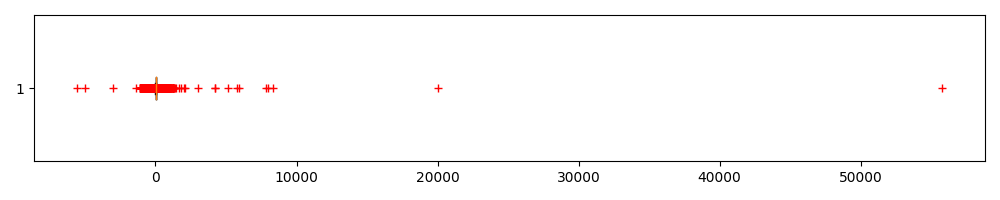
\includegraphics[width=\textwidth]{Task01.png}
\end{center}

\newpage
\section*{Task 02}
\paragraph{(a)}Below is a histogram with 50 bins distributed evenly across the range of the data. In this from the histogram is almost useless because of the extreme outliers contained in the data. \\
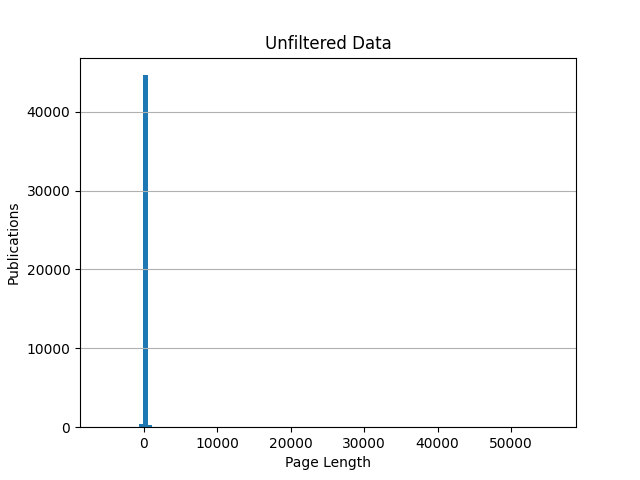
\includegraphics[width=\textwidth]{task02hist01.png}

\paragraph{(b)} The first class of data removed were articles with a page length of more than 50. This class consists of 797 entries, and roughly 1.7\% of the data. While this is not an insignificant amount, a page length of 50 places an article well into the 99th percentile of the data, and, as such, the data represents extreme outliers, but even more likely is incorrect. As can be seen in the histogram below, the histogram becomes much more compact, however, it is not yet to the point at which it can effectively show the patterns in the data. This is due to the fact that there are a number of data points that lie far into the negative pages numbers.

In terms of the statistical properties of the data, the upper and lower quartiles, as well as the median and minimum remain unchanged. The maximum logically becomes 50, and the mean falls from ~16.61 to ~6.37.

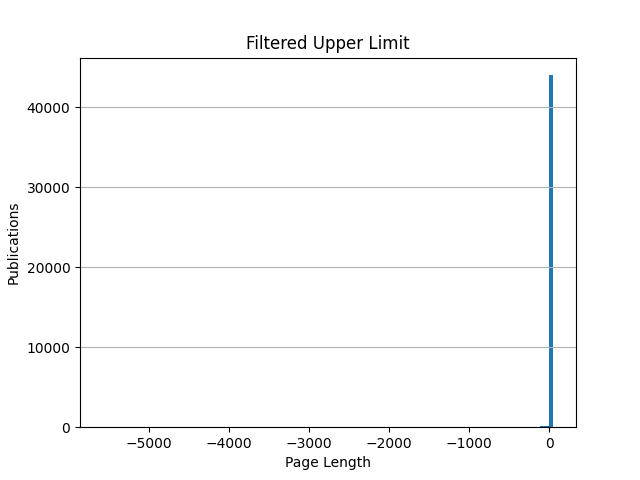
\includegraphics[width=\textwidth]{task02hist02.png}

The second class of data that was removed were the lines with page lengths less than 1. The reason for removing this class is relatively obvious; an article cannot consist of zero or less than zero pages. This class consists of 848 members and represents roughly 1.9\% of the data. The histogram below clearly shows that in this form, the data can be visualized much more effectively.

The changes in the statistical properties are similar to those seen in the previous filtering. Only the minimum and mean are affected, changing to 1 and ~9.62, respectively
	
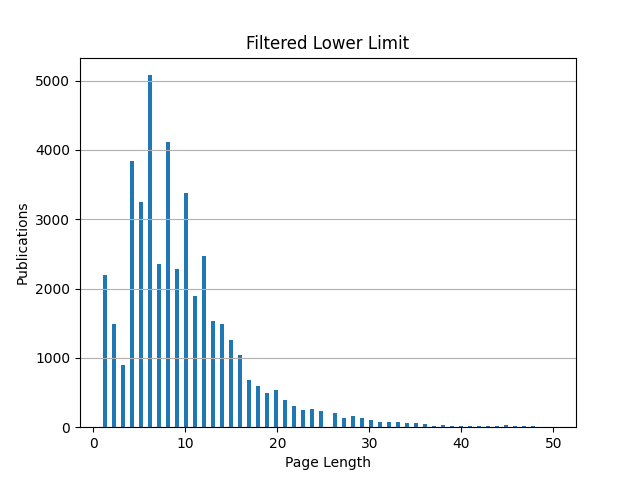
\includegraphics[width=\textwidth]{task02hist03.png}
	
	
\end{document}
















